\section{Architecture}

One of the important aspects of this study is to construct such an architecture that allows for the comparison of results between different models. Since the quality of predictions of models composed of various embedding methods and classification algorithms is being compared, it is necessary to ensure that the entire process is designed correctly. The individual variants of embeddings should be trained on the same data, and the classification algorithms on the same embeddings. Figure~\ref{methodology-schema_extended} illustrates the architecture designed for the purpose of comparing the results of the models in this study.

\begin{figure*}
\centering
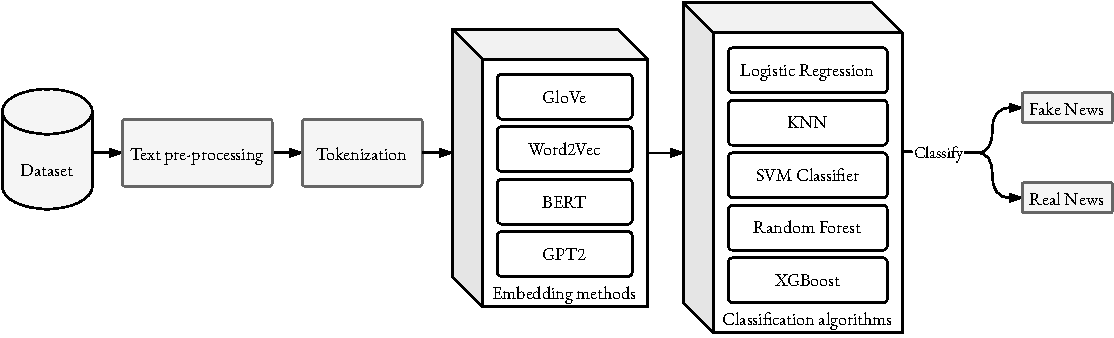
\includegraphics[width=0.95\linewidth]{methodology-schema_gpt2_extended.pdf}
\caption{Architecture of each embedding-classifier model combination}
\label{methodology-schema_extended}
\end{figure*}

The prepared dataset, previously subjected to cleansing and tokenization, has been divided into a training and testing set (further details regarding the dataset's characteristics are provided in the subsequent section). Subsequently, the data underwent an embedding procedure. The same combination of data was employed for all embedding methods utilized.

The Word Embeddings obtained in the previous step served as input for the classification algorithms in the subsequent step. After each word embedding procedure, each algorithm received exactly the same set of data. Hyperparameter tuning on the training set was performed using cross-validation with random search.

Finally, all combinations of 5 embedding methods and 6 classification methods resulted in 30 different fake news detection models. For each embedding-classifier combination, text classification into fake news and real news was performed on the test set created in the first step. More details about the obtained results will be presented in the Results section.

\section{Dataset}

Access to high-quality data is a significant challenge faced in data modeling and machine learning. In the absence of high-quality data, it is impossible to construct accurate machine learning models. Poor quality data, characterized by unreliable data collection methods, a large number of errors, incompleteness, or mislabeling, can compromise the effectiveness of any machine learning algorithm. This issue is particularly pertinent in the context of datasets containing fake news, where labeling is not as straightforward as with other datasets. The task of manual labeling, which is required to obtain ready-made texts labeled as fake news or real information, can be both time-consuming and challenging, requiring substantial trust in the person performing the labeling. As such, the labeling process is prone to significant human error, which can impact the selection of an appropriate dataset.

This research article aims to investigate how the use of various natural language processing (NLP) methods influences the accuracy of fake news prediction, rather than building a model to accurately predict fake news. Therefore, when selecting a dataset, the most crucial considerations are the quality of the labeled observations and the consistency of the labeled texts across the entire dataset. Additionally, the text should closely align with the research area, as the focus of this study is on detecting fake news. To construct a universal tool for detecting fake news, the dataset should include varied topics and text characteristics, reflecting the real-world distribution as accurately as possible. In this way, the model can learn from natural data, picking up the nuances present in different texts, such as writing style, formality, and topics. However, as noted earlier, the primary objective of this article is not to construct a ready-made tool but rather to examine and impact the predictive quality of different NLP methods. 

The dataset selected for the research that meets the above criteria is the \href{https://huggingface.co/datasets/liar}{LIAR} dataset, a publicly available dataset for detecting fake news presented by Wang in his 2017 paper. The dataset consists of 12,800 manually labeled texts collected from POLITIFACT.COM. These texts are characterized by different contexts, and each of them has been verified by POLITIFACT.COM editors. The texts have been labeled into 6 fine-grained labels evaluating the degree of truthfulness of the text: \textit{pants-fire}, \textit{false}, \textit{barely-true}, \textit{half-true}, \textit{mostly-true}, and \textit{true} \autocite{wang-2017-liar}.

In the context of this paper, I do not deal with multi-class classification. Instead, I reduce the number of classes to two, classifying \textit{true} and \textit{mostly-true} and \textit{half-true} as true news, and the remaining as fake news. As a result, I obtain a binary classification of text into true news and fake news. In the training set, 5,104 observations are classified as fake news compared to 6,420 pieces of information classified as true. In the test set, there are 553 fake news and 714 true news.  Both the training and test sets have a similar ratio of the two classes. I arbitrarily acknowledge that such a ratio of two classes is sufficient for conducting the study, and I do not undertake any further steps to improve data balance.


Next, I subjected the raw dataset to the process of data cleaning and feature engineering. The topics of the news articles were concatenated with their respective content, resulting in a longer text that retains all pertinent information. The cleaned texts were further processed by removing stopwords and punctuation marks. The topic information was omitted from the analysis as it unnecessarily complicates the dataset, potentially introduces uncertainty regarding its correctness, and is difficult to obtain for new data. Importantly, introducing additional variables would add noise to the prediction results, thereby complicating the analysis of the impact of different embedding methods on prediction accuracy. Similarly, the time variable of article publication was also omitted. The prepared dataset is now primed for subsequent analysis and the application of advanced embedding techniques to effectively process and represent the news content. % to ostatnie zdanie niekoniecznie w tek formie (styl) - zrobione

\section{Embeddings}

The next step after cleaning the data is to convert it in a way that is understandable to the computer. Textual data have the characteristic of forming a coherent whole. Individual letters form words, words form sentences, and sentences form longer pieces of text with a logical structure. Natural language is full of nuances. The same words can have different meanings and emotional connotations depending on the context. Understanding language comes naturally to humans and does not pose major difficulties. The human brain easily captures the appropriate context of words and their meaning, combining them into a logical and coherent text.

However, computers operate in a completely different way than the human brain. Computers are only capable of analyzing sequences of bits, which when arranged in a specific order, yield a result in the form of an element of a larger whole. This way, a sequence of bits can be presented as individual letters. Further, a sequence of letters can be represented as words. Then, in the tokenization process, individual words can be assigned a specific number. This way, the computer is able to decode the data represented by these words into something it can understand.

Nevertheless, the problem of conveying a deeper understanding of the text, the meaning of individual words, and the semantic relationships between them as understood in terms of similarity and analogies, still remains to be solved. The answer to this problem is Word Embedding. Word Embedding is used to represent words using numerical vectors, in such a way that the distance calculated between two words that are semantically similar is small, and between two semantically different words is large.

The Figure~\ref{embedding_example} illustrates the graphical interpretation of Word Embedding, often encountered in the literature. Similar words, such as King and Queen, Man and Woman, are closer to each other in the vector space. Two dimensions can be interpreted. The first dimension determines the fact of being a member of the family, while the second dimension indicates gender.

\begin{figure}[hbt!]
\centering
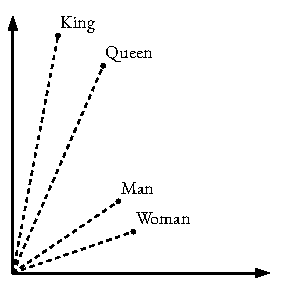
\includegraphics[width=0.4\linewidth]{embedding_example.pdf}
\caption{Similar words are closer together}
\label{embedding_example}
\end{figure}

Trained unsupervised machine learning algorithms handle the conversion of words into vectors from large sets of textual data. These algorithms learn to predict the context of a given word by analyzing the words with which it is associated. In this process, they learn the context of words and the semantic relationships between them. Examples of such algorithms include BERT, Glove, Word2Vec, and GPT-2, which has not yet been investigated in the literature for the purpose of fake news detection.

\subsection{GloVe}
GloVe (Global Vectors) is an unsupervised machine learning algorithm aimed at creating word embeddings by aggregating co-occurrence matrices of words that contain information about how often individual word pairs occur in a given text corpus.

The starting point is to create a co-occurrence matrix. The values in this matrix indicate how often a given word pair occurs together. The next step is to calculate the probability of one word occurring in the presence of another word, or rather the ratio between successive probabilities \autocite{Pennington2014}. Without delving into mathematical details, word embeddings are obtained using a matrix subjected to factorization in a process similar to dimensionality reduction \autocite{Albrecht2020}.

It is possible to use pre-trained word vectors trained on large text datasets. In this paper, a model trained on Common Crawl was used, consisting of 840 billion tokens and 2.2 million words, which allowed for obtaining 300-dimensional vectors for each word.

\subsection{Word2Vec}
The Word2Vec algorithm is yet another method for obtaining word embeddings. Unlike GloVe method, it is not a method that consists of a single, homogeneous algorithm. Word2Vec can be based on two distinct models: the CBOW and Skip-Gram Model.

The functioning of these two algorithms can be intuitively interpreted as two opposites. CBOW works as a model that predicts a given word based on its context. On the other hand, the Skip-Gram Model is a model that predicts the context of a given word, i.e., the words preceding and following it. Both models are built on a 3-layer neural network with an input layer, a hidden layer, and an output layer.

The originator of the Word2Vec method recommends using the Skip-Gram Model with negative sampling, which outperforms other variants in research. In this study, pre-trained vectors were used, trained on a portion of the Google News dataset consisting of about 100 billion words. The model consists of 300-dimensional vectors for 3 million words and phrases. It was not specified which Word2Vec method was used to obtain these vectors \autocite{Mikolov2013}.

\subsection{BERT}
BERT (Bidirectional Encoder Representations from Transformers) is a deep learning Large Language Model founded on the transformer self-attention mechanism. The transformer architecture incorporates encoders responsible for assimilating input data and assigning importance weights to individual words via the self-attention mechanism. This allows BERT to acquire an understanding of contextual dependencies among words within a sentence. Unlike sequential directional models, which process textual input data in a linear fashion, transformer encoders simultaneously process all words, resulting in an inherently bidirectional nature \autocite{Vaswani2017}. The bidirectional sentence-level classification architecture of BERT is depicted in the provided Figure~\ref{bert_architecture}.

\begin{figure}[hbt!]
\centering
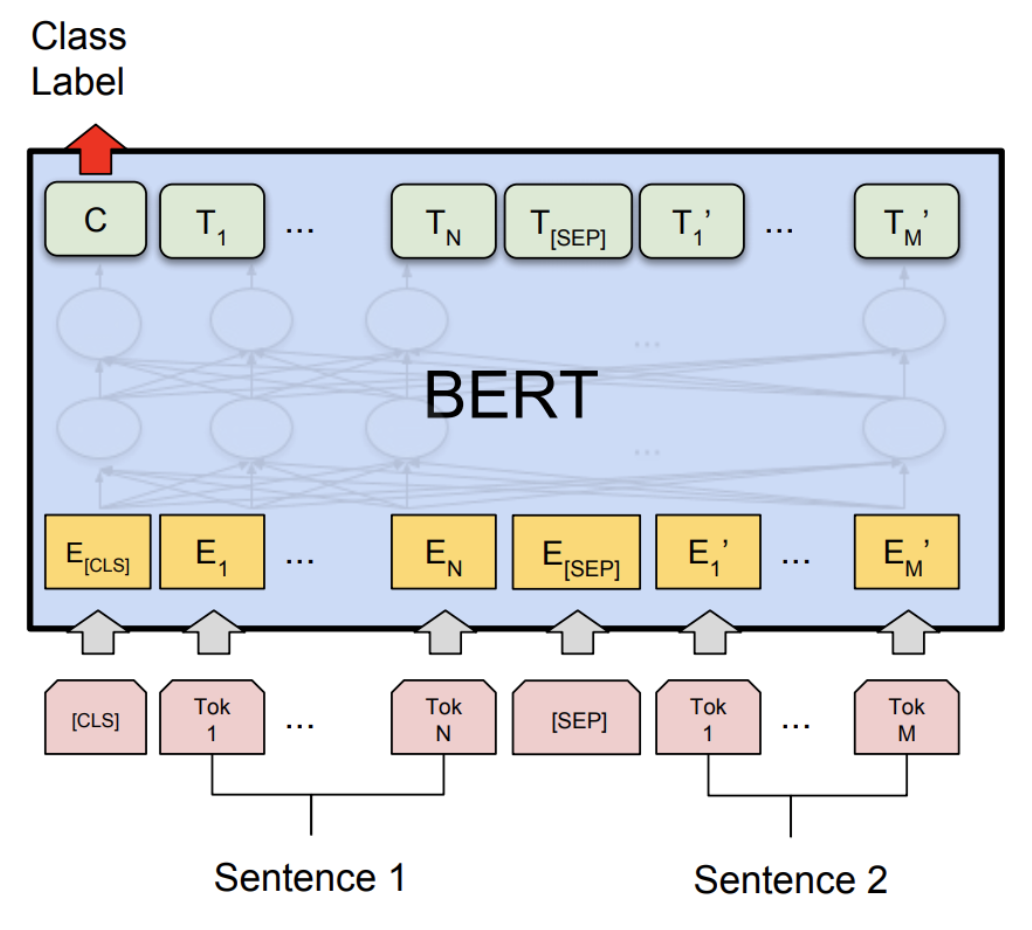
\includegraphics[width=0.6\linewidth]{bert_architecture.png}
\caption{BERT model architecture \autocite{Devlin2018}}
\label{bert_architecture}
\end{figure}

BERT belongs to the class of masked language models. This implies that the learning process of BERT can be interpreted in such a way that the model randomly masks a selected word and, based on the surrounding words (both preceding and succeeding), predicts the masked word using the mechanisms described earlier. 
Next Sentence Prediction (NSP) serves as another objective for the model during the pre-training process. In this procedure, BERT combines two randomly masked sentences as inputs. Subsequently, the model generates predictions regarding whether the given pair of sentences logically follows each other or not.

A noteworthy characteristic of BERT is its pre-training capability. During the pre-training phase, the BERT model acquires contextual understanding of a given word by analyzing the surrounding words. This is achieved through the application of a masked language model (MLM), where tokens are randomly masked, and the model attempts to predict the missing word's semantics. BERT offers a variety of pre-trained models that can be utilized for diverse purposes. Specifically, the BERT-base model, employed in this study, encompasses 12 encoder stack layers, 768 hidden units, and 12 multi-head attention heads, comprising a total of 110 million parameters. The pre-training of this model was conducted on a dataset containing 11,038 books and the English edition of Wikipedia.

BERT requires input data to be specially converted to the required format before being used in the pre-trained model. This enables the use of its key component, word embedding. During word embedding, BERT uses a technique called WordPiece. This technique is based on breaking words down into smaller subwords. This is done to capture the meanings of words that may have different interpretations or different meanings depending on the context. The WordPiece technique thus creates all combinations that can occur in a given text, assigning each extracted part a pre-trained vocabulary vector. These vectors then serve as input data for the previously trained transformer architecture.

An important feature of BERT is the fact that it can be fine-tuned for use in a specific task or adapted to the characteristics of a given dataset. Fine-tuning involves running the pre-trained model training on a new dataset for several epochs. According to the literature, such a trained model achieves state-of-the-art performance. However, in this paper, I will not be performing fine-tuning. Instead, I focus on comparing the impact of using different embedding methods on changes in model performance. Additionally, as mentioned earlier in the literature review, fine-tuning can be replaced by using a classifier on the pre-trained BERT architecture.

In this research, I use BERT as a feature extractor. I extract embeddings for the first token ([CLS] token) from the last hidden layer of the model.

\subsection{RoBERTa}
The Robustly Optimized BERT Approach (RoBERTa) is a modification of the BERT model. The creators of the model have modified the way in which the input data is masked. In the case of BERT, masked words were inputted to the model as input data. This is a weakness because during the training of the model in successive epochs, the model learned from the same duplicated data. RoBERTa introduces a change in the form of dynamic token masking during training in successive epochs. Additionally, another change introduced in RoBERTa is the removal of Next Sentence Prediction (NSP) during pre-training. The remainder of the architecture is identical to that of the BERT model.
Furthermore, RoBERTa is trained on a larger amount of data (160GB corpus text, with 16GB of the same data used for training BERT).
Due to the improvements made, RoBERTa is expected to demonstrate better performance than BERT \autocite{Liu2019}.

\subsection{GPT-2}
Another model utilizing the transformer architecture is the GPT-2 (Generative Pre-trained Transformer 2) model. Unlike BERT, it does not process input data in two directions but rather employs a unidirectional architecture that reads data from left to right. Another distinction is that GPT-2 utilizes decoder-only transformers (while BERT employed encoder-only transformers). This difference arises from the distinct purposes of the models. BERT was designed as a tool to create various models for different applications at a low cost by adding an additional layer. Consequently, BERT employs encoders whose output comprises contextualized embeddings that can serve as inputs for further models. On the other hand, GPT-2 serves an entirely different purpose, which is text generation. Since the model's output should be comprehensible to humans, GPT-2 relies solely on decoder-only transformers.

Decoders in GPT-2, similar to BERT, employ self-attention mechanisms. However, unlike BERT, self-attention in GPT-2 only takes into account preceding words. Otherwise, if considering the subsequent words in the sequence, the model would incorrectly learn to predict the next word by simply returning the next word in the sequence with the highest probability of occurrence. Another difference between GPT-2 and BERT lies in the fact that GPT-2 processes data token by token (while BERT processes the entire text simultaneously). GPT-2 generates predictions for the next word based on the preceding text. The output of one iteration simultaneously serves as the input for the next iteration.


\section{Classification algorithms}
The final component of the fake news detection model architecture is a classifier, which outputs only one of two values, namely whether a given sentence is a fake news or not. Classifiers are models whose results belong to previously defined classes, namely binary classification when there are two possible return values, or multiclass classification when there are more possible classes. There are many types of classifiers, which differ in structure and purpose depending on the characteristics of the data to which they are applied. Some classifiers perform better with one type of data than others. In selecting a group of classifiers for the study, I aimed to cover the widest range of popular classification models. Thus, logistic regression, which is a representative of econometric approach, K-Nearest Neighbours (KNN) and Support Vector Machine Classifier (SVC), which are representatives of non-parametric models, Random Forest as a representative of ensemble methods that use decision trees, eXtreme Gradient Boosting (XGBoost) as a representative of ensemble methods that use boosting, and neural networks, which are a separate class of models also widely used in classification, were chosen for the study.

\subsection{Logistic Regression}
Logistic Regression is a model used for binary classification. This model is based on the utilization of the logistic function to model the relationship between the variables in the model and the probability of the occurrence of a true event. The output of the model ranges from 0 to 1, which can be interpreted as the probability that a given observation is positive.

The logistic regression model is fitted by optimizing a loss function (in this case, the cross-entropy loss). In the optimization process, the aim is to obtain weights for the input variables (or parameters) that minimize the difference between the estimated probabilities and the actual values in the training set.

The logistic regression model can also be tuned. By having a set of variables, one can make choices about which variables are most useful in modeling a particular phenomenon, thereby minimizing model overfitting and improving its generalization. This is achieved through a technique called regularization. It introduces a "penalty" for the model for assigning larger weights to variables, thus "encouraging" the simplification of the model by eliminating the excessive influence of unnecessary variables. Two types of regularization are distinguished: L1 (Lasso Regularization) and L2 (Ridge Regularization). The key difference between them is that L1 regularization allows for the possibility of reducing weights to zero, completely eliminating variables from the model. On the other hand, L2 regularization does not allow for such a possibility, as variables always retain some nonzero weight. Additionally, it is possible to adjust the strength of the regularization. By selecting appropriate parameters, it is possible to find an optimal trade-off between the complexity of the model and its generalization.

Logistic regression is a parametric model that is based on certain a priori assumptions about the input data. The model assumes a linear relationship between the variables and the log-odds of positive classes (this assumption can be relaxed by introducing new variables that are combinations of the remaining ones).

\subsection{K-Nearest Neighbors (KNN)}
K-Nearest Neighbors (KNN) is an algorithm that can be used for both classification and regression tasks. It is non-parametric, meaning that no assumptions about the data are made during the fitting process. Instead, the data is directly used for making predictions. KNN operates on the principle that similar observations belong to the same classes. Upon receiving a new instance, the algorithm calculates the distance to the remaining observations and selects the K closest neighbors (hence the name of the algorithm). The new instance is then assigned to the cluster with which it shares the most common points, or in the case of regression, the mean is calculated.

Model tuning involves adjusting the number of neighbors (K) considered by the algorithm. Selecting an appropriate number of clusters is crucial because a too low value of K can lead to overfitting and high noise in the data. On the other hand, a large number of neighbors can make it difficult to capture local variations in the data.

To improve the model's performance, one can also customize the method used to calculate distances between instances. The most popular distance calculation methods include Euclidean distance, Manhattan distance, and Minkowski distance. It is important for accurate distance calculation that the variable ranges are similar. Therefore, it is important to normalize the variables prior to training KNN models.

\subsection{Support Vector Machine Classifier (SVC)}
Another popular algorithm used for both regression and classification is Support Vector Machine (SVM). The algorithm is based on finding the best possible hyperplane that separates the data into distinct classes. The constructed hyperplane aims to be as far as possible from two different data points belonging to different classes (these points are called support vectors), while minimizing the classification error. To achieve this, the hinge loss function is minimized, which penalizes the algorithm for misclassified observations.

By utilizing the Kernel Trick and mapping the data to a higher-dimensional space, SVM gains the ability to capture nonlinear relationships between variables. The most popular kernel functions include linear, polynomial, radial basis function (RBF), and sigmoid.

During SVM tuning, the parameter C can be modified, which influences the trade-off between maximizing the distance of the hyperplane from two different points and minimizing the classification error. A small value of the C parameter flattens the hyperplane, causing the model to potentially misclassify more points. A large value of the C parameter makes the hyperplane more prone to adjusting its shape to individual observations, while also exposing the model to overfitting.

\subsection{Random Forest}
Random Forest is a non-parametric algorithm that can successfully be used in both classification and regression tasks. It represents a family of ensemble methods, where the final predictions are the result of combining predictions from multiple decision trees. By leveraging the results of individual decision trees, Random Forest predictions are more accurate and robust. Each decision tree is estimated on randomly selected variables and observations selected with replacement. This technique, called bootstrap sampling, allows each decision tree to be trained on a slightly different dataset.

For each randomly selected subset of data, a decision tree is created, which iteratively divides the given dataset into two or more subsets. These divisions are made in such a way that the resulting groups differ as much as possible from each other. The degree of dissimilarity between subgroups can be measured, for example, using Gini impurity or information gain. Subsequent splits are generated until a stopping criterion is reached, such as maximum depth or minimum number of observations in a leaf node.

After creating all the trees, their predictions are combined into one. In the case of classification, this is done through majority voting, where the most frequently indicated value is selected.

In comparison to the previously described methods, Random Forest offers a larger number of hyperparameters for tunning. The most important ones include the number of trees, maximum depth, minimum samples split, and feature subset size. Modifying the number of trees in the forest usually involves a trade-off between model training cost and accuracy. The more trees, the more accurate the predictions, but at a higher prediction cost. The maximum depth of a tree determines its complexity level. Deeper trees capture variable dependencies better, but also increase the risk of overfitting. The minimum samples split parameter determines the minimum number of observations required to make a split. A smaller value results in a more complex tree. Modifying the feature subset size parameter affects the level of randomness and diversity among individual trees.

Due to its ability to handle multidimensional data, handle missing data, and provide feature importance, Random Forest is a common choice for creating machine learning models.

\subsection{eXtreme Gradient Boosting (XGBoost)}
The eXtreme Gradient Boosting (XGBoost) algorithm is another non-parametric algorithm based on the concept of decision trees. It is known for its high performance and effectiveness across a wide range of tasks. Similar to Random Forest, it represents a family of ensemble methods, specifically gradient boosting.

XGBoost predictions are generated by combining the predictions of multiple weak-performing models (typically decision trees) into a single strong model. The decision trees are created sequentially, and each subsequent tree is estimated based on the error of the previous tree, aiming to improve it by minimizing the loss function. As the name suggests, XGBoost utilizes the gradient boosting algorithm, which employs gradient descent optimization to minimize the loss function. In each iteration step, the algorithm computes the gradient of the loss function based on the predictions and updates the model by training the next tree on the residuals from the previous tree.

The idea of hyperparameter tuning in XGBoost is very similar to that of Random Forest. Just like in Random Forest, users can adjust the maximum depth of the trees, the number of trees in the ensemble, regularization parameters, and subsampling ratio. Changing the hyperparameters yields similar results as in Random Forest. Additionally, one can modify the learning rate, which refers to the speed at which subsequent models follow the gradient, effectively reducing the error of the previous model. A too high learning rate may cause the model to skip the global minimum of the gradient and settle for a local minimum, leading to overfitting. Conversely, a too low learning rate results in slower convergence, prolonging the model's learning process. By modifying the loss function and applying a sigmoid transformation to the final predictions, the model can successfully be used for binary classification.

\subsection{Neural Network}
The neural network model is inspired by the functioning of the human brain in its architecture. Neural networks operate based on interconnected nodes called neurons, which collectively participate in data processing and prediction generation. Among all the models discussed above, Neural Networks have the most diverse range of applications in various fields. They can be applied to all tasks that were previously discussed for other models. Additionally, they can be used for image recognition and natural language processing, which were not possible with the previously mentioned models. Standard neural networks have a fixed number of parameters, representing a family of parametric models.

The process of training neural networks consists of two main components: forward propagation and backpropagation. During forward propagation, the input data pass through the network and undergo computations layer by layer. Each neuron in the network transforms the data using adjustable activation functions and learnable parameters such as weights and biases. This process continues until the data traverse the entire network, reaching the output layer and obtaining predictions.

After obtaining predictions, the next step is to compare them with the true values and calculate the prediction error (or loss function). Subsequently, in the backpropagation process, this error is propagated in the reverse direction, from the output layer to the input layer. During backpropagation, the weight and bias of each neuron are adjusted using the gradient of the loss function, aiming to minimize the final error. The entire process can be repeated multiple times to optimize the model's performance. One such iteration (a complete pass of forward propagation and backpropagation) is called an epoch.

Neural networks can be tuned in various ways. One of them is modifying the network architecture, such as adding or removing layers and adjusting the number of neurons in each layer. Dropout is a commonly used technique, where randomly selected neurons are omitted during the learning process, improving the model's generalization. Other regularization techniques, such as L1 and L2 regularization, aim to mitigate overfitting. Similar to XGBoost, learning rate can be adjusted in neural networks. It functions analogously to XGBoost, determining how quickly a given model converges.

After appropriately adjusting the network architecture, it can successfully be utilized for classification tasks. The output layer can use activation functions like softmax to convert the output into probability values for different classes.


\section{Results}
Utilizing the architecture described in the previous section, I built separate models for each combination of embedding and classification algorithms. To verify the research hypotheses, it was necessary to examine the performance of each model thoroughly.

Since the study operated on a slightly imbalanced dataset, closer attention had to be paid to the issue of selecting appropriate metrics. Not all metrics are suitable for use on imbalanced data. In this case, an example of an incorrect metric would be accuracy. Accuracy is calculated as the ratio of correctly classified samples to the total number of samples, regardless of the class distribution. Therefore, when one class predominates numerically over the other, the model can achieve high accuracy simply by assigning all predictions to the majority class, thus making poor predictions on the less numerous class.

In the case of imbalanced data, a much better choice would be to use metrics such as Balanced Accuracy, F1 Score, or AUC-ROC, which were employed in this study.

Balanced Accuracy is a metric that deals with imbalanced classes by introducing a balanced evaluation of the model's performance on each class. It is the average percentage of true positive results that have been correctly classified (in other words, recall or sensitivity) for each class. However, Balanced Accuracy does not take into account precision, which focuses on the ratio of correct positive classifications. Depending on the goal we want to achieve when building a model, we may be interested in different metrics. For example, precision is crucial when the priority is to minimize false positives.

Another metric that can be successfully used to measure the performance of a model on an imbalanced dataset is the F1 Score. The F1 Score is the harmonic mean of precision and recall. It introduces a balance between precision and recall, which is useful when we want to consider both false positives and false negatives. The F1 Score takes values in the range of 0 to 1, with values closer to 1 indicating a better model. This metric is useful when assigning equal weight to the consequences of false positives and false negatives. Since I am looking for a metric that best compares performance while disregarding the business aspects of the model (such as modifying cutoff points to achieve a specific outcome), I consider it an appropriate metric for comparing models in this study.

The Area Under the Receiver Operating Characteristic Curve (AUC-ROC) measures the performance of a classification model. The ROC curve is a graphical representation of the tradeoff between true positive rate and false positive rate for different cutoff points. Similar to the F1 Score, it takes values between 0 and 1, where 1 denotes a perfect model, and 0.5 denotes a model that is no better than random. It is worth noting, however, that the AUC-ROC result is an average value across all threshold levels. Since this study focuses only on the default threshold level of 0.5, I choose the F1 Score as the leading and decisive metric for selecting the best model.

\begin{table}[htb]
\centering
\begin{tabular}{l|c|c|c|c|c}
\hline

% OLD
%\multicolumn{2}{c|}{\multirow{2}{*}{Model}} & \multicolumn{2}{c}{Score} \\
%\cline{3-4}
%\multicolumn{1}{l}{} & & Accuracy & F1-Score\\

% NEW
\multicolumn{2}{c|}{Model} & \multicolumn{4}{c}{Score} \\
\cline{1-6}
Embedding & Classification & Accuracy & B. Accuracy & F1 Score & ROC AUC \\

\hline
\multirow{6}{*}{GloVe}
    & Logistic Regression & 60.1 & 58.4 & 49.3 & 58.4 \\
    & KNN & 55.3 & 53.9 & 45.5 & 53.9 \\
    & SVM Classifier & 59.2 & 57.9 & 50.3 & 57.9 \\
    & Random Forest & 60.0 & 58.4 & 49.9 & 58.4 \\
    & XGBoost & 61.2 & 59.3 & 49.7 & 59.3 \\
    & Neural Network & 60.6 & 60.2 & \textbf{55.7} & 60.2 \\
\hline
\multirow{6}{*}{Word2Vec}
    & Logistic Regression & 61.7 & 59.7 & 49.9 & 59.7 \\
    & KNN & 54.0 & 53.4 & 47.9 & 53.4 \\
    & SVM Classifier & 60.5 & 59.4 & 53.0 & 59.4 \\
    & Random Forest & 57.9 & 56.1 & 46.6 & 56.1 \\
    & XGBoost & 57.1 & 56.0 & 48.7 & 56.0 \\
    & Neural Network & 60.6 & 59.9 & \textbf{54.6} & 59.9 \\
\hline
\multirow{6}{*}{BERT} 
    & Logistic Regression & 60.5 & 58.9 & 50.7 & 58.9 \\
    & KNN & 55.9 & 54.9 & 48.3 & 54.9 \\
    & SVM Classifier & 58.6 & 57.4 & 50.3 & 57.4 \\
    & Random Forest & 57.6 & 45.7 & 45.7 & 55.7 \\
    & XGBoost & 59.4 & 58.0 & 50.1 & 58.0 \\
    & Neural Network & 58.8  & 57.8 & \textbf{53.7} & 57.8 \\
\hline
\multirow{6}{*}{RoBERTa} 
    & Logistic Regression & 60.1 & 58.9 & 52.0 & 58.9 \\
    & KNN & 56.9 & 55.9 & 49.2 & 55.9 \\
    & SVM Classifier & 61.5 & 60.2 & 53.1 & 60.2 \\
    & Random Forest & 59.1 & 57.0 & 46.5 & 57.0 \\
    & XGBoost & 58.3 & 57.1 & 49.7 & 57.1 \\
    & Neural Network & 62.0 & 61.0 & \textbf{54.8} & 61.0 \\
\hline
\multirow{6}{*}{GPT-2} 
    & Logistic Regression & 62.0 & 60.6 & 53.6 & 60.6 \\
    & KNN & 55.2 & 53.4 & 43.4 & 53.4 \\
    & SVM Classifier & 61.6 & 60.1 & 52.2 & 60.1 \\
    & Random Forest & 58.8 & 57.0 & 47.8 & 57.0 \\
    & XGBoost &  60.1 & 58.6 & 50.6 & 58.6 \\
    & Neural Network & 60.3 & 59.7 & \textbf{54.6} & 59.7 \\
\hline
%\multicolumn{2}{c|}{Total Variables}     & 28,946 & 356 & 21,443 & 23,962\\
%\multicolumn{2}{c|}{Residual Error Mean} & 3.04   & 3.50 & 2.92  & 2.93 \\
%\hline
\end{tabular}
\caption{Results table}
\label{results_table}
\end{table}

Analyzing the results, I conclude that none of the models proved to be better than the best model presented by Khan et al. (55.7 vs. 62.0 F1 Score). However, the goal of this study was not to build the best-performing model but to compare how different tools affect the model's performance. When analyzing the embedding methods, it is difficult to determine if any of the methods turned out to be the best. To verify the hypothesis that language models outperform the other embedding methods used in this study, I employed the Kruskal-Wallis test. This test compares the medians of multiple independent groups and determines whether they are dependent on each other or not. This test does not assume data normality and can be used to compare groups of different sizes.

The results of the Kruskal-Wallis test indicate that the performance of different embedding models does not differ significantly from each other. The p-value of the Kruskal-Wallis test was 0.98 at a significance level of 0.05. Therefore, there is no basis for rejecting the null hypothesis that the median performance scores of individual embedding methods differ from each other.

The research hypothesis that language models (BERT, RoBERTa, GPT-2) outperform the other embedding methods (Word2Vec, GloVe) was not confirmed.

To verify the second null hypothesis that some classification algorithms perform better than others, I conducted a similar test among different classification methods.
The p-value of the Kruskal-Wallis test was <0.001 (=0.0002) at a significance level of 0.05. Therefore, the null hypothesis that the median performance scores of individual embedding methods differ from each other can be rejected.

The research hypothesis that the choice of classification algorithm significantly affects the model's results has been confirmed statistically.
However, the Kruskal-Wallis test does not indicate which of the examined groups differs from the others. To determine which group differs from the others, it would be necessary to perform pairwise comparisons between the groups.

%\begin{table}[htb]
%\centering
%{
%\makegapedcells
%\begin{tabular}{cc|cc}
%\multicolumn{2}{c}{}
%            &   \multicolumn{2}{c}{Predicted} \\
%    &       &   Yes &   No              \\ 
%    \cline{2-4}
%\multirow{2}{*}{\rotatebox[origin=c]{90}{Actual}}
%    & Yes   & 331   & 487                 \\
%    & No    & 165    & 284                \\ 
%    \cline{2-4}
%    \end{tabular}
% }
%\caption{Confussion matrix for the GPT-2+KNN model}
%\label{gpt2knn_cm}
%\end{table}


\begin{table}[htb]
\centering
{
\makegapedcells
\begin{tabular}{lll}
                & Predicted negative & Predicted positive \\
\hline
Actual negative & 454 (TN)           & 260 (FP) \\
Actual positive & 239 (FN)           & 314 (TP) \\
\hline
\end{tabular}
}
\caption{Confussion matrix for the GloVe+Neural Network model}
\label{glovenn_cm}
\end{table}

Upon analyzing the confusion matrix, it can be concluded that the best model successfully identified the majority of fake news and true news, exhibiting a relatively high number of true positives (TP) and true negatives (TN), while having a relatively low number of false positives (FP) and false negatives (FN).